\documentclass[aspectratio=169,10pt]{beamer}

% ==============================================================================
% THEME & STYLING CONFIGURATION
% ==============================================================================
\usetheme{Madrid}
\usecolortheme{whale}

\definecolor{sparshPurple}{RGB}{108, 99, 255}
\definecolor{sparshTeal}{RGB}{0, 201, 167}
\definecolor{sparshDark}{RGB}{15, 12, 41}
\definecolor{sparshAccent}{RGB}{255, 184, 0}

\setbeamercolor{palette primary}{bg=sparshPurple, fg=white}
\setbeamercolor{palette secondary}{bg=sparshDark, fg=white}
\setbeamercolor{palette tertiary}{bg=sparshTeal, fg=white}
\setbeamercolor{structure}{fg=sparshPurple}
\setbeamercolor{title}{bg=sparshPurple, fg=white}
\setbeamercolor{frametitle}{bg=sparshPurple, fg=white}
\setbeamercolor{block title}{bg=sparshPurple!20, fg=sparshPurple}
\setbeamercolor{block body}{bg=sparshPurple!5, fg=black}

\setbeamertemplate{navigation symbols}{}
\setbeamertemplate{footline}[frame number]

\usepackage{graphicx}
\usepackage{booktabs}
\usepackage{tabularx}
\usepackage{tikz}
\usetikzlibrary{positioning, arrows.meta}

% ==============================================================================
% TITLE & METADATA
% ==============================================================================
\title[SPARSH Pitch Deck]{\textbf{SPARSH: AI-Powered Multi-Sensory Inclusive Learning Platform}}
\subtitle{Bridging the Education Gap for Visually, Hearing, and Physically Impaired Learners}
\author[Dravida Developers]{\textbf{Team Dravida Developers}\\Aqib Majeed (Team Leader) \quad Saqib Ahmad (Core Member)\\[0.15cm]\small \textbf{Project Guide:} Sona G, Assistant Professor (CSE)}
\institute[GCE Tirunelveli]{Government College of Engineering, Tirunelveli -- 627 007\\[0.1cm]\textbf{NMNT Project ID: NMNTSTD950061}}
\date{Academic Year 2025--2026}

\begin{document}

% ------------------------------------------------------------------------------
% SLIDE 1: TITLE SLIDE
% ------------------------------------------------------------------------------
\begin{frame}
    \titlepage
\end{frame}

% ------------------------------------------------------------------------------
% SLIDE 2: THE PROBLEM
% ------------------------------------------------------------------------------
\begin{frame}{The Global Crisis: Educational Exclusion}
    \begin{columns}[T]
        \begin{column}{0.48\textwidth}
            \begin{block}{\textbf{2.2+ Billion Individuals Globally}}
                \begin{itemize}
                    \item Experience visual, hearing, or physical disabilities.
                    \item In India alone, over \textbf{6.8 million children with disabilities} struggle for basic educational access.
                    \item Drop-out rates in inclusive schools exceed \textbf{60\%} due to the lack of personalized sensory aids.
                \end{itemize}
            \end{block}
        \end{column}
        \begin{column}{0.48\textwidth}
            \begin{block}{\textbf{The Failure of Conventional Tools}}
                \begin{itemize}
                    \item \textbf{Commercial Braille Displays:} Prohibitive cost ranging from \textbf{Rs.~1,60,000 to Rs.~4,00,000+} per device.
                    \item \textbf{Textbook Media:} Formatted strictly for sighted readers; zero native tactile haptic integration.
                    \item \textbf{Language Isolation:} Modern speech engines favor standard English, ignoring Indic regional dialects.
                \end{itemize}
            \end{block}
        \end{column}
    \end{columns}
\end{frame}

% ------------------------------------------------------------------------------
% SLIDE 3: OUR SOLUTION
% ------------------------------------------------------------------------------
\begin{frame}{The SPARSH Solution: Multi-Sensory Inclusive Ecosystem}
    \begin{center}
        \textbf{SPARSH converts standard national curriculum content simultaneously into:}\\[0.2cm]
        \textbf{\textcolor{sparshPurple}{Visual}} \quad $\bullet$ \quad 
        \textbf{\textcolor{sparshTeal}{Auditory}} \quad $\bullet$ \quad 
        \textbf{\textcolor{orange}{Tactile (Haptic)}} \quad $\bullet$ \quad 
        \textbf{\textcolor{blue}{Gestural (ISL)}}
    \end{center}
    \vspace{0.2cm}
    \begin{columns}[T]
        \begin{column}{0.5\textwidth}
            \begin{block}{\textbf{Affordable Hardware Suite (Rs.~2,850)}}
                \begin{itemize}
                    \item \textbf{SPARSH Smart Glove:} 5-finger flex gesture recognition.
                    \item \textbf{SPARSH Smart Glasses:} VLM live scene OCR.
                    \item \textbf{SPARSH SenseBand:} Multi-profile haptic wristband.
                    \item \textbf{SPARSH Smart Keyboard:} 28-key diode-less matrix.
                \end{itemize}
            \end{block}
        \end{column}
        \begin{column}{0.5\textwidth}
            \begin{block}{\textbf{Intelligent Software Platform (Rs.~0 Free)}}
                \begin{itemize}
                    \item \textbf{VoiceVision Assistant:} "Hello Sparsh" wake word.
                    \item \textbf{Braille Lab:} Instant A4 tactile PDF converter.
                    \item \textbf{Sign Lab:} 3D articulated ISL Avatar.
                    \item \textbf{SPARSH Duo:} Gamified blind/deaf learning track.
                    \item \textbf{NCERT AI RAG:} 17,800+ national textbook chapters.
                \end{itemize}
            \end{block}
        \end{column}
    \end{columns}
\end{frame}

% ------------------------------------------------------------------------------
% SLIDE 4: HARDWARE INNOVATIONS & BOM PRICING
% ------------------------------------------------------------------------------
\begin{frame}{Hardware Engineering: Complete Ecosystem Under Rs.~2,850}
    \begin{table}[htbp]
        \centering
        \renewcommand{\arraystretch}{1.25}
        \resizebox{\textwidth}{!}{%
        \begin{tabular}{|l|p{6.4cm}|c|}
            \hline
            \textbf{Assistive Device} & \textbf{Key Engineering Innovation} & \textbf{Unit Price (INR)} \\ \hline
            \textbf{SPARSH Smart Glove} & 12-bit ADC flex mapping (70--200 counts) + 100\,ms deflection heuristics & Rs.~1,150 \\ \hline
            \textbf{SPARSH Smart Glasses} & ESP32-CAM OV2640 with multimodal VLM scene description \& OCR & Rs.~680 \\ \hline
            \textbf{SPARSH SenseBand} & Dual LRA vibration + active-low synchronized buzzer (5 modes) & Rs.~480 \\ \hline
            \textbf{SPARSH Smart Keyboard} & 28-key diode-less matrix with active lockout ghost suppression & Rs.~540 \\ \hline
            \textbf{Total Ecosystem} & \textbf{Complete 4-Peripheral Hardware Suite} & \textbf{Rs.~2,850} \\ \hline
        \end{tabular}%
        }
    \end{table}
    \vspace{0.15cm}
    \begin{center}
        \textcolor{sparshTeal}{\textbf{Result: More than 98\% cost reduction compared to commercial assistive products (Rs.~1,60,000+).}}
    \end{center}
\end{frame}

% ------------------------------------------------------------------------------
% SLIDE 5: SYSTEM ARCHITECTURE & PRICING
% ------------------------------------------------------------------------------
\begin{frame}{Three-Tier Decoupled Architecture \& Cost Breakdown}
    \begin{center}
        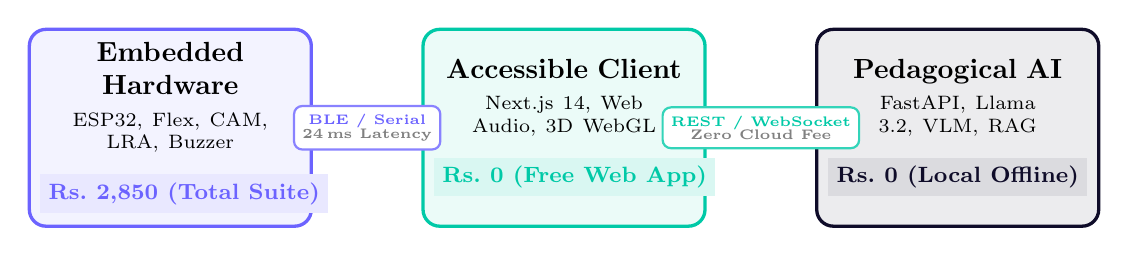
\begin{tikzpicture}[
            tierBox/.style={
                draw=#1, 
                fill=#1!8, 
                line width=1.2pt, 
                rounded corners=6pt, 
                text width=3.3cm, 
                minimum height=2.5cm, 
                align=center, 
                inner sep=4pt
            },
            connectorBadge/.style={
                draw=#1!80, 
                fill=white, 
                line width=0.8pt, 
                rounded corners=3pt, 
                align=center, 
                inner sep=3pt, 
                font=\tiny\bfseries
            }
        ]
            % --- Tier 1: Embedded Hardware ---
            \node[tierBox=sparshPurple] (hw) at (-5.0, 0) {
                \textbf{\normalsize Embedded Hardware}\\[0.12cm]
                \scriptsize ESP32, Flex, CAM, LRA, Buzzer\\[0.22cm]
                \colorbox{sparshPurple!15}{\textbf{\footnotesize\textcolor{sparshPurple}{Rs.~2,850 (Total Suite)}}}
            };

            % --- Tier 2: Accessible Client ---
            \node[tierBox=sparshTeal] (client) at (0, 0) {
                \textbf{\normalsize Accessible Client}\\[0.12cm]
                \scriptsize Next.js 14, Web Audio, 3D WebGL\\[0.22cm]
                \colorbox{sparshTeal!15}{\textbf{\footnotesize\textcolor{sparshTeal}{Rs.~0 (Free Web App)}}}
            };

            % --- Tier 3: Pedagogical AI ---
            \node[tierBox=sparshDark] (ai) at (5.0, 0) {
                \textbf{\normalsize Pedagogical AI}\\[0.12cm]
                \scriptsize FastAPI, Llama 3.2, VLM, RAG\\[0.22cm]
                \colorbox{sparshDark!15}{\textbf{\footnotesize\textcolor{sparshDark}{Rs.~0 (Local Offline)}}}
            };

            % --- Connections with guaranteed spacing & clean badges ---
            \draw[<->, line width=1.5pt, sparshPurple] (hw.east) -- (client.west)
                node[midway, connectorBadge=sparshPurple] {
                    \textcolor{sparshPurple}{BLE / Serial}\\[-1pt]
                    \fontsize{5}{6}\selectfont\textcolor{gray}{24\,ms Latency}
                };

            \draw[<->, line width=1.5pt, sparshTeal] (client.east) -- (ai.west)
                node[midway, connectorBadge=sparshTeal] {
                    \textcolor{sparshTeal}{REST / WebSocket}\\[-1pt]
                    \fontsize{5}{6}\selectfont\textcolor{gray}{Zero Cloud Fee}
                };
        \end{tikzpicture}
    \end{center}
    
    \vspace{0.15cm}
    \begin{columns}[T]
        \begin{column}{0.48\textwidth}
            \begin{block}{\textbf{Zero Recurring Cost Philosophy}}
                \begin{itemize}
                    \item \textbf{100\% Free Software Stack:} No student subscriptions, SaaS paywalls, or per-query API bills.
                    \item \textbf{Offline Local Inference:} Llama 3.2 runs locally on commodity classroom PCs via Ollama.
                \end{itemize}
            \end{block}
        \end{column}
        \begin{column}{0.48\textwidth}
            \begin{block}{\textbf{Open-Source Hardware Advantage}}
                \begin{itemize}
                    \item \textbf{Rs.~2,850 Ecosystem:} 4 complete assistive peripherals for less than the cost of a single textbook.
                    \item \textbf{Driverless Chrome Access:} Plug-and-play Web BLE and Web Serial connectivity.
                \end{itemize}
            \end{block}
        \end{column}
    \end{columns}
\end{frame}

% ------------------------------------------------------------------------------
% SLIDE 6: SOFTWARE HIGHLIGHTS
% ------------------------------------------------------------------------------
\begin{frame}{Software Innovations: Purpose-Built Accessibility}
    \begin{columns}[T]
        \begin{column}{0.48\textwidth}
            \begin{block}{\textbf{VoiceVision AI Engine}}
                \begin{itemize}
                    \item \textbf{Web Audio Synthesizer:} Zero-latency chime cues ($523\,\text{Hz} \rightarrow 880\,\text{Hz}$) for state changes.
                    \item \textbf{Autonomous Wake Word:} "Hello Sparsh" greeting with hands-free command execution.
                    \item \textbf{Continuous Loop:} Barge-in TTS suppression prevents echo feedback.
                \end{itemize}
            \end{block}
            \begin{block}{\textbf{Braille Lab \& PDF Generator}}
                \begin{itemize}
                    \item Bidirectional English \& Bharati Braille mapping.
                    \item Instant printable/embossing A4 PDF worksheet creation with cell-by-cell dot matrices.
                \end{itemize}
            \end{block}
        \end{column}
        \begin{column}{0.48\textwidth}
            \begin{block}{\textbf{Sign Lab: 3D ISL Avatar}}
                \begin{itemize}
                    \item 5-digit articulated hand joints with organic flutter.
                    \item SLERP quaternion bone interpolation.
                    \item Single-pass animation execution (no loop glitch).
                \end{itemize}
            \end{block}
            \begin{block}{\textbf{SPARSH Duo Gamification}}
                \begin{itemize}
                    \item Duolingo-style gamified levels tailored for sensory impairments.
                    \item Computer vision webcam verification for sign practice.
                    \item Streak counters, XP rewards, and haptic feedback.
                \end{itemize}
            \end{block}
        \end{column}
    \end{columns}
\end{frame}

% ------------------------------------------------------------------------------
% SLIDE 7: COMPETITIVE ADVANTAGE
% ------------------------------------------------------------------------------
\begin{frame}{Competitive Advantage Matrix}
    \begin{table}[htbp]
        \centering
        \renewcommand{\arraystretch}{1.22}
        \resizebox{\textwidth}{!}{%
        \begin{tabular}{|l|c|c|c|c|}
            \hline
            \textbf{Feature / Capability} & \textbf{Commercial Braille} & \textbf{Speech Apps} & \textbf{Duolingo} & \textbf{SPARSH Platform} \\ \hline
            \textbf{Hardware Suite Cost} & Rs.~1,60,000--Rs.~4,00,000 & Rs.~50,000+ (Device) & Smartphone only & \textbf{Rs.~2,850 (All 4 Peripherals)} \\ \hline
            \textbf{Multi-Sensory Modalities} & Tactile only & Audio only & Visual only & \textbf{4 Modalities (Synchronized)} \\ \hline
            \textbf{Sign Language (ISL) Avatar} & None & None & None & \textbf{Articulated 3D (SLERP)} \\ \hline
            \textbf{Automated Tactile PDF Export} & Limited & None & None & \textbf{Instant A4 Worksheets} \\ \hline
            \textbf{Indian Regional Languages} & Very Rare & Limited & Hindi only & \textbf{Tamil, Hindi, English} \\ \hline
            \textbf{Curriculum Integration} & None & None & None & \textbf{17,800+ NCERT Chapters} \\ \hline
            \textbf{Open-Hardware Architecture} & Proprietary & Proprietary & Proprietary & \textbf{100\% Open Source (ESP32)} \\ \hline
        \end{tabular}%
        }
    \end{table}
    \vspace{0.1cm}
    \begin{center}
        \small\textcolor{sparshTeal}{\textbf{SPARSH is the only platform providing full tactile hardware, 3D ISL avatar, and NCERT RAG.}}
    \end{center}
\end{frame}

% ------------------------------------------------------------------------------
% SLIDE 8: TARGET MARKET & PRICING STRUCTURE
% ------------------------------------------------------------------------------
\begin{frame}{Target Market \& Transparent Pricing Structure}
    \begin{columns}[T]
        \begin{column}{0.48\textwidth}
            \begin{block}{\textbf{Transparent Pricing Packages}}
                \begin{itemize}
                    \item \textbf{Individual Student Kit:} \textbf{Rs.~2,850}\\
                    Includes Smart Glove, Smart Glasses, SenseBand, Smart Keyboard, and full software access.
                    \item \textbf{Inclusive Classroom Lab Pack (10 Sets):} \textbf{Rs.~28,500}\\
                    10 complete peripheral sets + institutional teacher analytics dashboard.
                    \item \textbf{Software \& AI Curriculum:} \textbf{Rs.~0 (Free Forever)}\\
                    Public digital infrastructure supporting NEP 2020.
                \end{itemize}
            \end{block}
        \end{column}
        \begin{column}{0.48\textwidth}
            \begin{block}{\textbf{Target Market in India}}
                \begin{itemize}
                    \item \textbf{1.5 Million+ Public Schools:} Covered under Government of India \textit{Samagra Shiksha Abhiyan}.
                    \item \textbf{3,200+ Special Education Centers:} Serving visually and hearing impaired learners.
                    \item \textbf{Rural \& Low-Income Students:} Who cannot afford commercial Rs.~1,60,000+ displays.
                \end{itemize}
            \end{block}
        \end{column}
    \end{columns}
\end{frame}

% ------------------------------------------------------------------------------
% SLIDE 9: TEAM & RECOGNITION
% ------------------------------------------------------------------------------
\begin{frame}{Team Dravida Developers: Mission-Driven Engineers}
    \begin{columns}[T]
        \begin{column}{0.48\textwidth}
            \begin{block}{\textbf{Core Engineering Team}}
                \begin{itemize}
                    \item \textbf{Aqib Majeed (Team Leader):}\\Full-Stack Architecture, AI Inference, Web Speech, and Embedded C++.
                    \item \textbf{Saqib Ahmad (Core Member):}\\Hardware Circuitry, Sensor Calibration, FreeRTOS Firmware, and 3D Modeling.
                    \item \textbf{Sona G (Faculty Supervisor):}\\Assistant Professor, Dept. of CSE, Government College of Engineering, Tirunelveli.
                \end{itemize}
            \end{block}
        \end{column}
        \begin{column}{0.48\textwidth}
            \begin{block}{\textbf{Project Credentials}}
                \begin{itemize}
                    \item \textbf{NMNT Project ID:} NMNTSTD950061
                    \item \textbf{Institutional Affiliation:} Government College of Engineering, Tirunelveli (Anna University).
                    \item \textbf{Dataset Validation:} 17,800+ NCERT national textbooks cataloged with live RAG inference.
                \end{itemize}
            \end{block}
        \end{column}
    \end{columns}
\end{frame}

% ------------------------------------------------------------------------------
% SLIDE 10: CONCLUSION & LIVE DEMO
% ------------------------------------------------------------------------------
\begin{frame}{Summary: Every Voice Matters, Every Child Learns}
    \begin{center}
        \vspace{0.4cm}
        {\Huge \textcolor{sparshPurple}{\textbf{SPARSH}}}\\[0.2cm]
        {\Large \textit{Sensory Pedagogical AI Resource for Special Education}}\\[0.6cm]
        
        \begin{beamercolorbox}[sep=8pt,center,rounded=true,shadow=true]{palette tertiary}
            \textbf{\Large Experience the Live Multi-Sensory Demo}
        \end{beamercolorbox}
        
        \vspace{0.4cm}
        \textbf{Smart Glove \quad $\bullet$ \quad Smart Glasses \quad $\bullet$ \quad SenseBand \quad $\bullet$ \quad Braille Lab}\\[0.3cm]
        {\small Government College of Engineering, Tirunelveli $\bullet$ Team Dravida Developers}\\[0.1cm]
        {\footnotesize Contact: Aqib Majeed \& Saqib Ahmad}
    \end{center}
\end{frame}

\end{document}
